\subsubsection{Giao diện chính của ứng dụng}
\hspace*{2em} Hình ~\ref{fig:main-interface} minh họa giao diện chính sau khi người dùng đăng nhập thành công.  
Tại đây, ứng dụng chia thành ba mục chính: \textbf{Bạn bè}, \textbf{Nhóm} và \textbf{Hội thoại}, giúp người dùng dễ dàng quản lý các mối quan hệ và cuộc trò chuyện.  
Giao diện được thiết kế nhất quán với tông màu chủ đạo xanh lam và các biểu tượng trực quan mang lại trải nghiệm sử dụng đơn giản và thân thiện.  

\begin{figure}[H]
  \centering
  \begin{minipage}{0.32\textwidth}
    \centering
    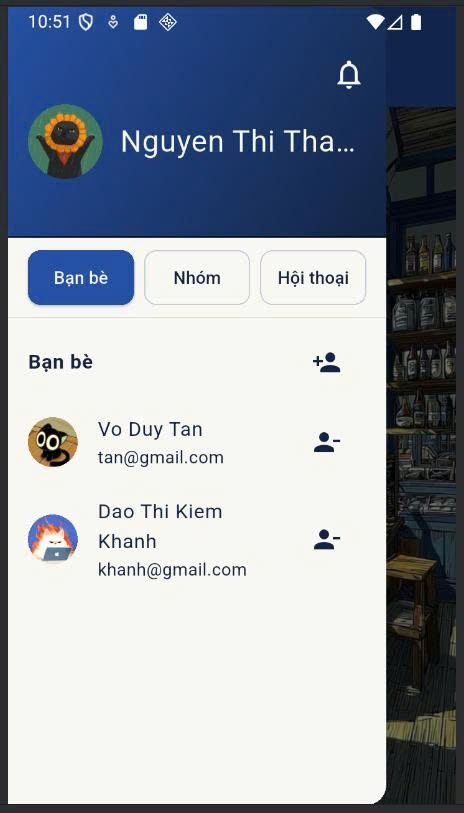
\includegraphics[width=\textwidth]{figures/pic11(1).jpg}
    \caption*{(a) Danh sách bạn bè}
  \end{minipage}
  \hfill
  \begin{minipage}{0.32\textwidth}
    \centering
    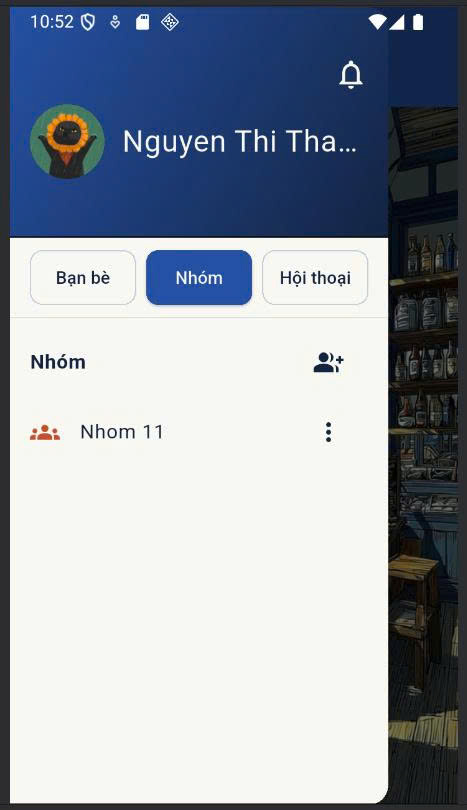
\includegraphics[width=\textwidth]{figures/pic11(2).jpg}
    \caption*{(b) Danh sách nhóm}
  \end{minipage}
  \hfill
  \begin{minipage}{0.32\textwidth}
    \centering
    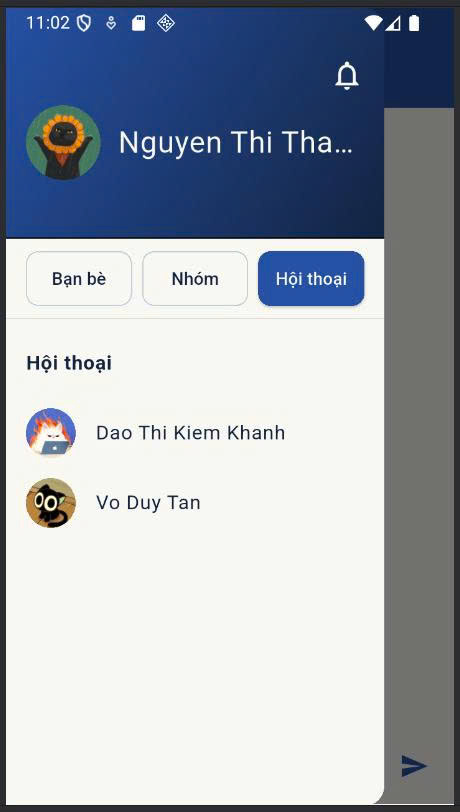
\includegraphics[width=\textwidth]{figures/pic11(3).jpg}
    \caption*{(c) Danh sách hội thoại}
  \end{minipage}
  \caption{Giao diện chính gồm các mục: bạn bè, nhóm và hội thoại.}
  \label{fig:main-interface}
\end{figure}
